\chapter{Understanding datasets}

\section{Source of the data}

\subsection{Barkley Earth}

Berkeley Earth is independent, non-profit organization founded by Richard and Elizabeth Muller in 2010, focused on environmental data sience and analysis. 
One of the main purposes of the project is to raise awareness about global warming. 
Berkeley Earth provides open source air polution and global temperature data \cite{berkeleyearthdata}. 
Their datasets cover 250 years of the Earth temperature.
\\Berkeley Earth publishes their data in two type of formats
\begin{itemize}
    \item Time Series Data
    \item Gridded Data
\end{itemize}

{\it Time Series Data} summarises tabular format of yearly, monthly and daily anomalies of land's temperature. 
Below there is an example of such representation
\begin{verbatim}
%               Monthly    Annual    Five-year  Ten-year   Twenty-year
% Year, Month,  Anomaly,   Anomaly,  Anomaly,   Anomaly,   Anomaly
  ...
  1987     1     0.587     0.255     0.270      0.339      0.344
  1987     2     1.008     0.249     0.274      0.344      0.345
  1987     3     0.017     0.300     0.281      0.353      0.346
  1987     4     0.300     0.323     0.287      0.354      0.347
  ...
\end{verbatim}

{\it Gridded Data} adds additional dimension to a dataset. A grid is represended in two forms, as 1º x 1º {\it latitude-longitude} representation or {\it Equal Area} format that divides the Earth into 15984 equaled cells.
When analyzing data and predicting the Earth's temperature fluctuations with machine learning models, Time Series Data will be employed.

\subsection{Our World in Data}
Our World in Data is a project of the Global Change Data Lab, a non-profit organization based in the United Kingdom.
Our World in Data’s mission is to publish the \textit{research and data to make progress against the world’s largest problems}.
The datasets accessible on ourworldindata.org cover a wide range of topics, including, but not limited to, environmental changes, food, agriculture, education and knowledge, and health, as referenced in \cite{ourworldindata}.

\section{Datasets Insights}

\subsection{Temperature anomalies}

Majority of the tempoerature measurements use 1951 - 1980 period as a baseline. There are a couple of factors behind this decision. Firstly, this period wasn't affected so mutch by Green House Gass emission. 
Secondly, in this time there were no major vulcanic erruptions and solar disturbances, that could affect the Earth's temperature. Another argument for using the period between 1951 - 1980, accordin to NASA, is
``We choose 1951-1980 as the base period because that was the base period at the time that 'global warming' began to be a public issue. Also it is the time that 'baby boomers' grew up, so this choice for base period allows those people to relate today's climate to that which they remember`` \cite{nasa-giss}.
Both figures ~\ref{fig:temperature_anomalies} and ~\ref{fig:climat_stripes} clearly visualize temperature anomalies trends since 1820.

\begin{figure}[h]
  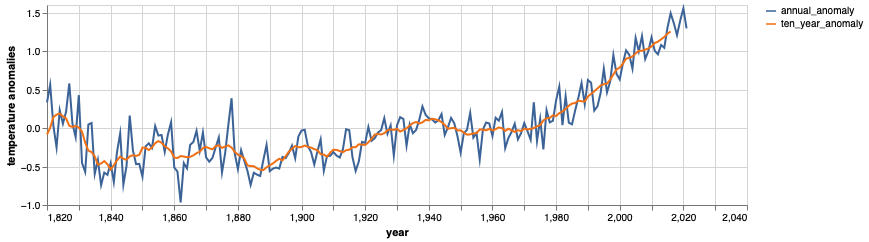
\includegraphics[width=\linewidth]{img/temperature_anomalies.png}
  \caption{Land temperature anomalies since 1820}
  \label{fig:temperature_anomalies}
\end{figure}

\begin{figure}[h]
  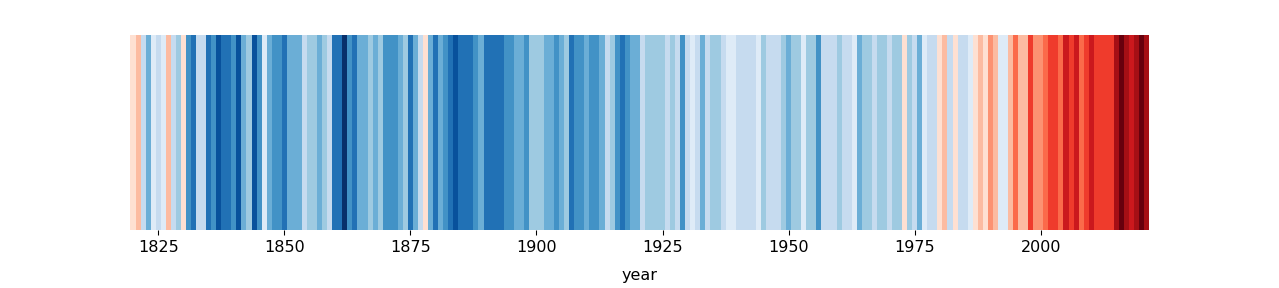
\includegraphics[width=\linewidth]{img/climate_stripes.png}
  \caption{Land climate stripes since 1820}
  \label{fig:climat_stripes}
\end{figure}

\subsection{\coo\ emission}

Based on the dataset, total quantity of emmited \coo\ since 1750 year, was 11,912,250 million metric tons. 
Figure ~\ref{fig:co2_emission_global} illustrates the fluctuations of carbon dioxide emissions across different countries in 1800, 1850, 1900, 1950, 2000, and 2020.
\begin{figure}[h]
  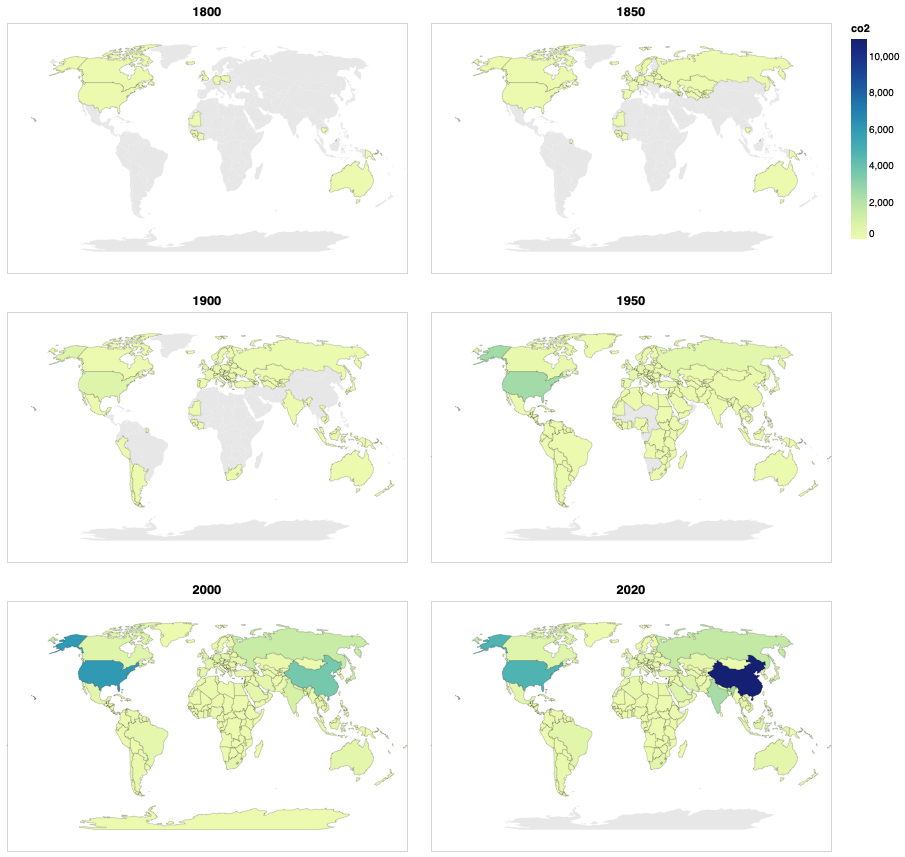
\includegraphics[width=\linewidth]{img/co2emission.png}
  \caption{The figure illustrates the amount of \coo\ emissions during six distinct time periods and is a static representation of an interactive image developed for the project .For further details, refer to \cite{github}. Lack of data is represented by gray color areas.} 
  \label{fig:co2_emission_global}
\end{figure}

\newpage 
On the other hand, chart ~\ref{fig:co2_emission_by_region} demonstrates \coo\ emission since 1750. 
Notably, Europe and the USA were the primary contributors to these emissions until the year 2000. 
According to the report \cite{why-are-greenhouse-gases-decreasing}, EU countries have experienced a significant reduction in emission due to a 
\begin{itemize}
  \item decrease in fossil fuel combustion
  \item lowering the energy consumption and improving energy efficiency
  \item increased adoption of renewable energy sources
\end{itemize}
However, it is noteworthy that despite having signed the Paris Agreement with the goal of limiting global warming to 1.5°C, China has yet to take significant action to reduce its greenhouse gas emissions. While China has announced a new goal to achieve carbon neutrality by 2060, it has emerged as a leading contributor to global \coo\ emissions in recent years.
\newline
Overall, it is hoped that all countries will take concerted and effective measures to reduce their greenhouse gas emissions in order to mitigate the impacts of climate change and limit global warming to manageable levels.

\begin{figure}[h]
  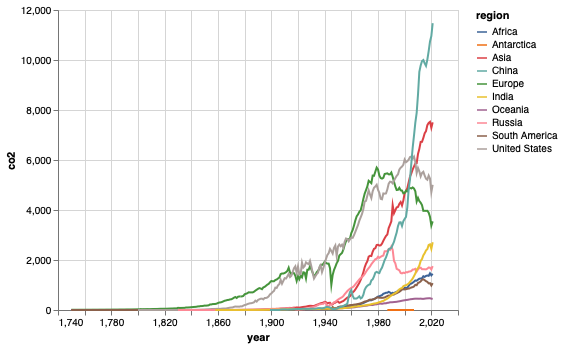
\includegraphics[width=\linewidth]{img/co2emission_by_region.png}
  \caption{Carbon dioxide emission since 1800 year grouped by continents. China, Russia, Indie and United States of America are represented by independent lines}
  \label{fig:co2_emission_by_region}
\end{figure}

There are numerous factors that can contribute to carbon dioxide emissions. According to the Parson's correlation table shown in ~\ref{tab:correlations-co2-pop-gdp}, it can be inferred that there is a positive correlation between GDP and \coo\ emissions.
Similarly, a comparable trend for European Union countries was observed in \cite{relation-between-co2-gdp}.

\begin{table}[ht]
\begin{tabular}{ |p{3cm}||p{2cm}|p{2cm}|p{2cm}|  }
 \hline
 & \textbf{population} & \textbf{gdp} & \textbf{co2} \\
 \hline
\textbf{population} &  1.000000 	& 0.587208 	& 0.597836 \\
  \textbf{gdp} &  0.587208  &	1.000000 &	0.922921  \\
  \textbf{co2} &  0.597836 &	0.922921 &	1.000000 \\
 \hline
\end{tabular}
\caption{Correlation table between \coo\ emission, population and gross domestic product for \coo\ emission dataset} 
\label{tab:correlations-co2-pop-gdp}
\end{table}

\subsection{Corelation between \coo\ emission and temperature anomalies}

Certainly, it is a natural question to ask about the correlation between \coo\ emissions and temperature anomalies. By combining both datasets and matching them by the year, we can gain valuable insights into this relationship. The use of a Parson's correlation table, see table ~\ref{tab:correlations-co2-annomalies}, helps to determine whether there is a significant correlation between the two variables.

\begin{table}[ht]
\begin{tabular}{ |p{3cm}||p{2,7cm}|p{3cm}|p{1,7cm}|  }
 \hline
 & \textbf{year anomaly} & \textbf{ten year anomaly} & \textbf{co2} \\
 \hline
\textbf{year anomaly} &  1.000000 &	0.934620 &	0.886943 \\
  \textbf{ten year anomaly} &  0.934620 &	1.000000 &	0.932080  \\
  \textbf{co2} &  0.886943 	& 0.932080 &	1.000000 \\
 \hline
\end{tabular}
\caption{Correlation table between \coo\ emission and temperature anomalies} 
\label{tab:correlations-co2-annomalies}
\end{table}

\begin{figure}[H]
  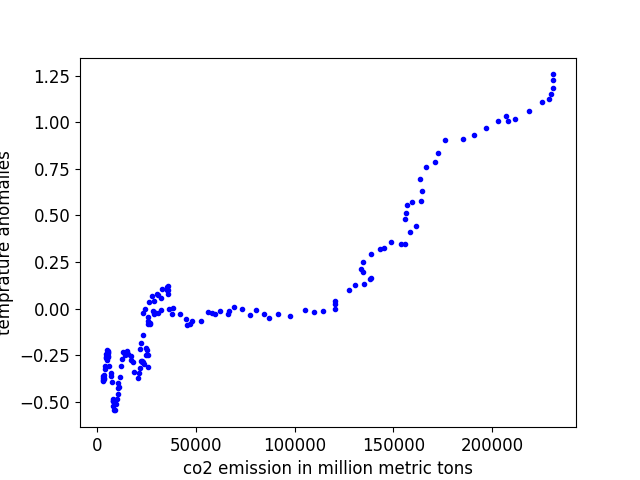
\includegraphics[width=\linewidth]{img/co2-temperature-corelation.png}
  \caption{Corelation between \coo\ emission and temperature anomalies}
  \label{fig:co2-temperature-corelation}
\end{figure}

\section{Summary}
According to Berkeley Earth \cite{berkeleyearthdata} the Earth has warmed up by 1.3\degree C.
Furthermore, the rising trend of \coo\ emissions from year to year has been identified as a significant contributing factor to the Earth's overall temperature increase. 
Figure ~\ref{fig:co2-temperature-corelation} demonstrates correlation between \textit{ten year anomaly} and \coo\ which will serve as an input for the machine learning methods used in \autoref{chap:two} to predict the Earth's temperature.
